% This is samplepaper.tex, a sample chapter demonstrating the
% LLNCS macro package for Springer Computer Science proceedings;
% Version 2.20 of 2017/10/04
%
\documentclass[runningheads]{llncs}
%
\usepackage{graphicx}
\usepackage[utf8]{inputenc}
\usepackage[brazil]{babel}
\usepackage{indentfirst}
\usepackage[pdftex]{hyperref}

% Used for displaying a sample figure. If possible, figure files should
% be included in EPS format.
%
% If you use the hyperref package, please uncomment the following line
% to display URLs in blue roman font according to Springer's eBook style:
\renewcommand\UrlFont{\color{blue}\rmfamily}

\begin{document}
%
\title{Verificação, Validação e Priorização de Requisitos}
%\titlerunning{Abbreviated paper title}
% If the paper title is too long for the running head, you can set
% an abbreviated paper title here
%
\author{Higor Dantas\inst{1}\orcidID{118110808},
Ivyna Alves\inst{2}\orcidID{115110057}, Matheus Justino\inst{3}\orcidID{118111780} e
Thaís Toscano\inst{4}\orcidID{115111596}}
%
\authorrunning{H. Dantas, I. Alves et al.}
% First names are abbreviated in the running head.
% If there are more than two authors, 'et al.' is used.
%
\institute{Universidade Federal de Campina Grande, Campina Grande - PB, Brasil
\email{higor.dantas@ccc.ufcg.edu.br} \and
\email{ivyna.alves@ccc.ufcg.edu.br} \and
\email{matheus.justino@ccc.ufcg.edu.br} \and
\email{thais.toscano@ccc.ufcg.edu.br}}
%
\maketitle              % typeset the header of the contribution
%
\begin{abstract}
Uma das dificuldades enfrentadas no desenvolvimento de software é entender bem os requisitos e, em seguida, reproduzí-los no sistema, já que a linguagem natural tem como forte característica a ambiguidade. Sendo assim, a compreensão de um requisito de forma errônea, traz grandes prejuízos para o projeto, já que fará que a equipe aloque mais tempo para modificar o que já foi implementado, perdendo assim, tempo de desenvolvimento. Dessa maneira, a utilização de estratégias de prioridade e verificação e validação de requisitos são importantes para o ciclo de vida de desenvolvimento do software, já que tem o objetivo de evitar tais erros. Diante disso, o trabalho a seguir mostrará estratégias para o elaboração do sistema de forma eficiente e segura.

\keywords{Verificação e validação  \and Requisitos \and Software.}
\end{abstract}
%
%
%
\section{Introdução}

\section{Verificação}
O principal papel dessa fase é observar se todos os requisitos funcionais e não-funcionais elucidados foram bem definidos, ou seja, não possuem ambiguidades, inconsistências e nem omissões. Logo, essa fase deve ser iniciada o quanto antes já que quanto mais adiantado o processo de desenvolvimento maior se torna o custo de realizar as devidas correções.

Para isso, deve-se ao longo dessa fase realizar algumas verificações nas documentações geradas:

\begin{itemize}
    \item \textbf{Verificações de validade}: Uma funcionalidade do sistema pode depender de uma outra funcionalidade adicional ou diferente da relatada pela documentação.
    \item \textbf{Verificações de consistência}: Uma funcionalidade não pode ter descrições diferentes ou restrições que se contradizem.
    \item\textbf{Verificações de completude}: O documento deve conter todas as funções, e suas devidas descrições, necessárias aos usuários do sistema.
    \item \textbf{Verificações de realismo}: Essa verificação é importante para passar a garantia de que todas funcionalidades descritas são possíveis de implementar, considerando o orçamento e o cronograma definido para o desenvolvimento do sistema.
    \item \textbf{Verificabilidade}: Essa atividade garante que é possível escrever casos de testes que cubram todos os requisitos definidos para o sistema. Isso ajuda, principalmente, na redução de conflitos entre o cliente e o contratante.
\end{itemize}

\section{Validação}
Segundo Ian Sommerville, finalidade da validação é assegurar que o sistema de software atenda às expectativas do cliente. Dessa maneira, esse processo representa a atividade em que obtemos o aceite do cliente sob determinado artefato. No cenário de engenharia de requisitos, esta atividade significa aprovar junto ao cliente os requisitos que foram especificados.

\section{Técnicas de Verificação e Validação}
As formas de realizar as validações e verificações de requisitos são divididas em duas categorias: estáticas e dinâmicas, de modo que está ultima se faz necessária para se ter o código em execução, diferentemente das estáticas, que não possui a dita funcionalidade. No tocante às atividades acima descritas, as referidas podem ser realizadas mediante a utilização de algumas técnicas, quais sejam as inspeções, os walkthroughs e os checklists.

\subsection{Verificação e Validação Estática}

\subsubsection{Inspeções}
Esse processo possui o objetivo de observar defeitos antes que a fase de testes tenha início, porém existem diversas formas de ser executada, a forma tradicional foi criada por Fagan, em 1976. Porém, ao longo dos anos esse modelo passou por diversas modificações e atualmente o ideal é que pelo menos 4 pessoas participem podendo desempenhar mais de um papel.

Os papéis são:
\begin{itemize}
    \item Autor: responsável pela descoberta de defeitos e suas correções.
    \item Inspetor: deve encontrar erros ou inconsistências nos artefatos separados para inspeção.
    \item Relator: registra os resultados das reuniões.
    \item Moderador: papel que realiza o gerenciamento e busca facilitar a realização das inspeções, além de planejar todas as atividades.
\end{itemize}

Nas versões mais atuais costuma ter 6 fases basicamente, são elas:
\begin{enumerate}
    \item \textbf{Planejamento}: O moderador define o contexto que ocorrerá a inspeção, seleciona os usuários que desempenharão o papel de inspetor e distribui o material que passará pela inspeção.
    \item \textbf{Detecção de defeitos}: Os inspetores selecionados anteriormente deve realizar uma atividade de detecção de defeitos, onde será produzido uma lista de desconformidades.
    \item \textbf{Coleção de Defeitos}: O moderador reúne todas as listas produzidas pelos inspetores no passo anterior e elimina as discrepâncias repetidas, já que podem ser relatadas por mais de um inspetor.
    \item \textbf{Discriminação de defeitos}: O moderador, o autor do documento e os inspetores realizam discussões das discrepâncias encontradas. Durante esse passo cada problema relatado receberá uma classificação entre falso positivo e defeito. Daí, os reais defeitos são repassados ao autor, que realizará as devidas correções.
    \item \textbf{Retrabalho}: O autor realiza as correções dos problemas relatados no passo anterior.
    \item \textbf{Continuação}: O autor repassa o material corrigido para o moderador, que irá realizar uma avaliação da necessidade de uma nova inspeção ou não.
\end{enumerate}

\begin{figure}[h]
    \centering
    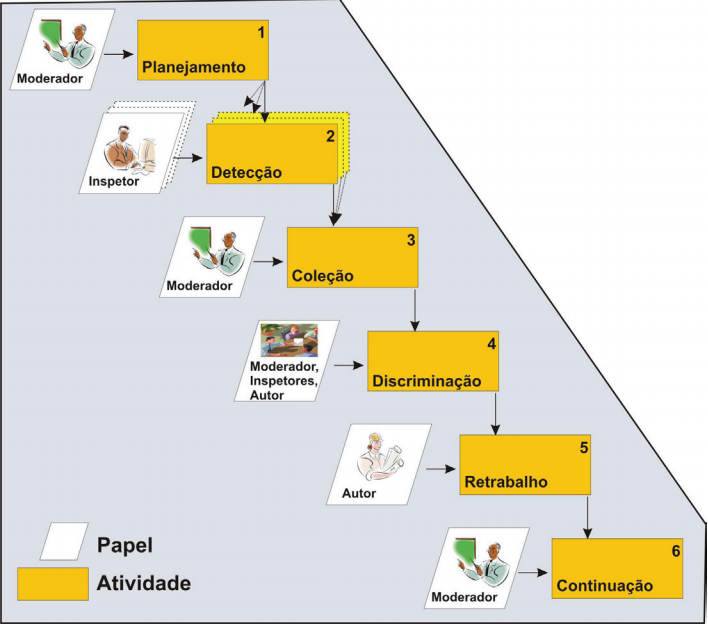
\includegraphics[width=10cm]{inspecao.png}
    \caption{Processo de Inspeção.}
    Fonte: \cite{ref_article1}.
    \label{fig:inspecao.png}
\end{figure}

\subsubsection{Walkthrough} É um processo menos rigoroso que o apresentado acima, onde costuma possuir de entre 3 e 5 participantes, com a possibilidade de desempenhar papel de autor, de líder de revisões ou de revisores.

O processo inicia selecionando uma parte do sistema que deverá passar por uma avaliação de no máximo 2 horas, onde cada revisor simula a execução passo a passo no papel para que se detecte algum erro. Porém, é uma técnica bastante desestruturada e para ser bem sucedida é necessário que a equipe tenha bastante dedicação e eficiência.

\subsection{Verificação e Validação Dinâmica}
Sua principal forma é por meio da execução de testes, onde se executa o programa com entradas específicas e verifica se o comportamento tá dentro do esperado.

A forma dinâmica busca responder, basicamente, três perguntas:

\begin{enumerate}
    \item \textit{Quando testar?} Está relacionado à fase de desenvolvimento.
        \begin{itemize}
            \item {Teste de unidade}: Consiste em testar a menor unidade.
            \item {Teste de integração}: Verifica se os componentes funcionam quando estão em conjunto.
            \item {Teste de sistema}: Avalia o software de forma integrada, como um usuário final.
            \item {Teste de aceitação}: São testes que verificam funcionalidade e verifica se as mesmas estão de acordo com o esperado.
            \item {Teste de regressão}: A cada nova versão do software deve-se executar todos os testes já realizados anteriormente.
        \end{itemize}
    \item \textit{O que testar?} Está relacionado com o tipo de teste que será realizado.
        \begin{itemize}
            \item {Teste de funcionalidade}: Testa os requisitos funcionais, de acordo com o documentado gerado inicialmente.
            \item {Teste de interface}: Verifica se a navegabilidade e os objetivos da tela funcionam como esperado.
            \item {Teste de desempenho}: Testa a capacidade de resposta do sistema a uma determinada solicitação.
            \item {Teste de carga}: Analisa o funcionamento da aplicação exercendo sobre ela uma quantidade grande de usuários ao mesmo tempo.
            \item {Teste de usabilidade}: Testa as questões que interfere na relação do sistema com o sistema (facilidade no uso, por exemplo).
            \item {Teste de volume}: Tem a função de testar a quantidade de dados envolvidos.
            \item {Teste de segurança}: Testa a segurança dos dados dos usuários da aplicação.
        \end{itemize}
    \item \textit{Como testar?} Utilizado quando se está preocupado apenas com as saídas ou com as estruturas internas.
        \begin{itemize}
            \item {Teste funcional da caixa-preta}: Usado quando a preocupação não é com o código produzido e sim com a saída esperada e obtida.
            \item {Teste estrutural caixa-branca}: É o oposto do anterior, representa preocupação com a estrutura interna do sistema.
        \end{itemize}
\end{enumerate}


\section{Priorização de Requisitos}

\subsection{Definição}
A priorização é uma forma de lidar com demandas conflitantes por recursos limitados. Estabelecer a prioridade relativa de cada capacidade de produto permite planejar a construção para fornecer o maior valor com o menor custo, com isso o mesmo ajuda o projeto a fornecer o máximo valor comercial o mais rápido possível dentro das restrições do projeto.

Até mesmo um projeto de tamanho médio pode ter dezenas de requisitos do usuário e centenas de requisitos funcionais. Para mantê-lo gerenciável, escolha um nível apropriado de abstração para a priorização - recursos, casos de uso, histórias de usuários ou requisitos funcionais. Dentro de um caso de uso, alguns fluxos alternativos podem ter uma prioridade mais alta que outros.

Alan Davis (2005) indica que a priorização bem sucedida requer uma compreensão de seis questões: As necessidades dos clientes; A importância relativa dos requisitos para os clientes; O momento em que as capacidades precisam ser entregues; Requisitos que servem como predecessores para outros requisitos e outros relacionamentos entre requisitos; Quais requisitos devem ser implementados como um grupo; O custo para satisfazer cada requisito.

Há requisitos que devem ser implementados juntos ou em uma sequência específica, pois não fará sentido implementar algo que não possa ser desfeito e/ou atualizado, por exemplo, você pode acabar escrevendo código para, digamos, aceitar pagamentos com cartão de crédito sem verificar se o cartão é válido, rejeitando cartões que foram relatados como roubados ou manipulando outras exceções.

\subsection{Técnicas}

Priorizar requisitos não é algo simples e devido a necessidade cada vez maior do uso de metodologias ágeis no desenvolvimento de softwares surgiram algumas técnicas que auxiliam nesse processo.

\subsubsection{In or Out}
É caracterizado pela formação de um grupo que tem interesse no projeto, o mesmo produz uma lista de requisitos e vão tomando decisões binárias: \textit{Este requisito está dentro ou fora?}

\subsubsection{Pairwise comparison and rank ordering}
O grupo envolvido no projeto atribui uma lista com uma sequência de prioridades exclusivas para cada requisito. Após concluída, faz-se comparações entre pares dentre todos eles, para que no final seja percebido qual membro de cada par tem maior prioridade.

\subsubsection{Three-level scale}
Essa abordagem de priorização agrupa os requisitos em três categorias: alta, média e baixa. Há alguns fatores para que sejam estabelecidos qual nível os requisitos estão. Os requisitos de alta prioridade são importantes e urgentes. Alternativamente, obrigações contratuais ou de conformidade podem ditar que um requisito específico deve ser incluído, ou pode haver razões comerciais convincentes para implementá-lo prontamente. Requisitos de prioridade média são importantes mas não são urgentes. Os requisitos de baixa prioridade não são importantes, nem urgentes, e ainda há uma quarta categoria onde diz que os requisitos parecem urgentes para alguns interessados, mas eles não são realmente importantes para alcançar os objetivos de negócios.\\

Ao executar uma análise de priorização com a escala de três níveis, você precisa estar ciente das dependências de requisitos. Você terá problemas se um requisito de alta prioridade depender de outro classificado com prioridade mais baixa e, portanto, planejado para implementação posteriormente.

\subsubsection{MoSCoW}
As quatro letras maiúsculas representam quatro possíveis classificações de prioridade para os requisitos em um conjunto (IIBA 2009): 

\begin{itemize}
    \item Must: O requisito deve ser satisfeito para que a solução seja considerada um sucesso;
    \item Should: O requisito é importante e deve ser incluído na solução, se possível, mas não é obrigatório para o sucesso;
    \item Could: É uma capacidade desejável, mas que pode ser adiada ou eliminada. Implemente-o somente se o tempo e os recursos permitirem;
    \item Won't: isso indica um requisito que não será implementado no momento, mas pode ser incluído em uma versão futura. 
\end{itemize}

Esse esquema altera a escala de três níveis para uma escala de quatro, ele não oferece nenhuma justificativa para tomar a decisão sobre como classificar a prioridade de um determinado requisito em comparação a outros. Ele também possui ambiguidade quanto ao tempo, particularmente quando se trata da classificação "Won't". "Não" pode significar "não no próximo lançamento" ou "nunca", com isso, esta técnica não é recomendada.

\subsubsection{\$100 (hundred-dollar)}
Esta técnica consiste em dar à equipe de priorização 100 dólares imaginários para trabalhar, os mesmos alocam esses dólares para “comprar” itens que eles gostariam de ter implementado do conjunto completo de requisitos do candidato. Eles ponderam os requisitos de prioridade mais alta alocando mais dólares a eles. Se um requisito for três vezes mais importante para um interessado do que outro requisito, ela atribui talvez nove dólares ao primeiro requisito e três dólares ao segundo, desta forma faz com que os participantes realizem suas próprias alocações de dólares e, em seguida, somem o número total de dólares atribuídos a cada requisito para ver quais deles, coletivamente, têm a prioridade mais alta.

\subsection{Priorização baseada em valor, custo e risco}

Uma maneira definitiva e rigorosa de relacionar o valor do cliente aos recursos do produto proposto é com uma técnica chamada Implantação da Função de Qualidade, ou QFD (Cohen 1995). 
Os participantes típicos no processo de priorização incluem o gerente de projetos ou analista de negócios, que lidera o processo, arbitra conflitos e ajusta os dados de priorização recebidos dos outros participantes, se necessário, e os representantes do cliente que fornecem as classificações de benefício e penalidade.

Representantes de desenvolvimento, que fornecem as classificações de custo e risco:

\begin{enumerate}
    \item Listar em uma planilha todos os recursos, casos de uso, fluxos de casos de uso, histórias de usuários ou requisitos funcionais que você deseja priorizar uns contra os outros. Usamos recursos no exemplo. Todos os itens devem estar no mesmo nível de abstração: não misture requisitos funcionais com recursos, casos de uso ou histórias de usuários.
    \item Classificar de 1 a 9 os benefícios relativos ao cliente de cada requisito (1 indica que ninguém consideraria útil; 9 significa que seria extremamente valioso).
    \item Classificar de 1 a 9 as penalidades caso aquele requisito não seja incluído no projeto (1 significa que ninguém ficará chateado se estiver ausente; 9 indica uma desvantagem séria).
    \item A planilha calcula o valor total de cada característica como a soma de suas pontuações de benefício e penalidade. A planilha soma os valores de todos os recursos e calcula a porcentagem do valor total que vem de cada um dos recursos (a coluna Valor\%).
    \item Classificar de 1 a 9 os custos relativos da implementação, pelos desenvolvedores, (1 -- rápido e fácil -- a 9 -- demorado e caro). Os desenvolvedores estimam as classificações de custo com base na complexidade do recurso, na extensão do trabalho da interface do usuário necessária, na capacidade potencial de reutilizar o código existente, na quantidade de testes necessária e assim por diante.
    \item Classificar de 1 a 9 o risco técnico relativo. O risco técnico é a probabilidade de não obter o recurso logo na primeira tentativa. Uma classificação de grau 1 significa que o risco é baixíssimo, enquanto que 9 indica sérias preocupações sobre a viabilidade, a falta de conhecimento necessário sobre a equipe, o uso de ferramentas e tecnologias desconhecidas, ou a preocupação com a quantidade de complexidade escondida dentro do requisito.
    \item Depois de inserir todas as estimativas na planilha, deve-se calcular um valor de prioridade para cada recurso usando a seguinte fórmula: 
        \begin{equation}
            priority = value\% / (cost\% + risk\%)
        \end{equation}
    \item Por fim, deve-se classificar a lista de recursos em ordem decrescente por prioridade calculada, a coluna mais à direita. Os recursos no topo da lista têm o balanço de valor, custo e risco mais favorável e, portanto, todos os outros fatores sendo iguais devem ter a prioridade mais alta. 
\end{enumerate}

A utilidade desse modelo de prioridade é limitada pela capacidade da equipe de estimar o benefício, a penalidade, o custo e o risco de cada item




%
% ---- Bibliography ----
%
% BibTeX users should specify bibliography style 'splncs04'.
% References will then be sorted and formatted in the correct style.
%
% \bibliography{mybibliography}
%
\bibliographystyle{splncs04}
\begin{thebibliography}{}
\bibitem{ref_book1}
Wiegers, K., Beatty, J.: Software Requirements. 3ª ed. (2013).

\bibitem{ref_book2}
Sommerville, Ian. Engenharia de software. 9ª ed. (2011).

\bibitem{ref_article1}
Engenharia de Software Magazine. Ano 1, 1ª ed (2007), 68 -- 74. Acesso em: \url{https://profandreluisbelini.files.wordpress.com/2016/02/revista-engenharia-de-software-ano-1-1c2ba-edic3a7c3a3o.pdf}

\bibitem{ref_article2}
Dos Santos, C. W.: PROCESSO DE V&V APLICADO AO DESENVOLVIMENTO DE SOFTWARE DO NTIC. Alegrete (2015). Acesso em: \url{http://dspace.unipampa.edu.br/bitstream/riu/859/1/Processo\%20de\%20V\%26V\%20aplicado\%20ao\%20desenvolvimento\%20de\%20software\%20do\%20NTIC.pdf}

\end{thebibliography}
\end{document}

